\documentclass[main.tex]{subfiles}
\usepackage{graphicx}
\usepackage{slashed}
\usepackage{color}
%\usepackage{amsmath}
%\usepackage{amssymb}

\definecolor{mypink}{RGB}{219, 48, 122}
\definecolor{mygreen}{rgb}{0,0.7,0}
\def\SB#1{\textcolor{mygreen}{{\bf\tt [SB: #1]}}}
\def\TP#1{\textcolor{yellow}{{\bf\tt [TP: #1]}}}
\def\BH#1{\textcolor{red}{{\bf\tt [BH: #1]}}}
\def\EC#1{\textcolor{mypink}{{\bf\tt [EC: #1]}}}
\def\SZ#1{\textcolor{blue}{{\bf\tt [SZ: #1]}}}
\def\JK#1{\textcolor{cyan}{{\bf\tt [JK: #1]}}}
\def\txB#1{\textcolor{blue}{#1}}

%%% spinor products %%%

\def\finite{\mathrm{finite}}
\def\renorm{\mathrm{ren,CDR}}
\def\irpole{\mathrm{pole,CDR}}
 
\def\fin{\mathrm{fin}}
\def\zz{\boldsymbol{Z}}
\def\mi{\mathrm{MI}}
\def\cF{\mathcal{F}}
\def\cP{\mathcal{P}}
\def\cC{\mathcal{C}}
\def\cA{\mathcal{A}}
\def\cN{\mathcal{N}}
\def\cO{\mathcal{O}}
\def\cD{\mathcal{D}}
\def\cQ{\mathcal{Q}}
\def\cJ{\mathcal{J}}
\def\cI{\mathcal{I}}
\def\cT{\mathcal{T}}
\def\nn{\nonumber \\ }

\def\wpol{\varepsilon_W}
\def\lrbrace#1{\lbrace#1\rbrace}
\def\la{\langle}
\def\ra{\rangle}
\def\spA#1#2{\la#1#2\ra}
\def\spB#1#2{[#1#2]}
\def\spAB#1#2#3{\la#1|#2|#3]}
\def\spBA#1#2#3{[#1|#2|#3\ra}
\def\spAA#1#2#3{\la#1|#2|#3\ra}
\def\spBB#1#2#3{[#1|#2|#3]}
\def\spab#1#2{\la#1|#2]}
\def\spaa#1#2#3#4{\la#1|#2|#3|#4\ra}
\def\spbb#1#2#3#4{[#1|#2|#3|#4]}
\def\wh#1{\widehat#1}
%\DeclareMathOperator{\tr}{\rm tr}
%\def\trm{\tr_-}
%\def\trp{\tr_+}
\def\MP#1#2{(#1\cdot#2)}
%\def\trfive{\tr_5}
\def\spAXB#1#2#3#4#5{\la#1|#2|#3|#4|#5]}

\def\bra#1{\langle #1|}
\def\ket#1{|#1 \rangle}
\def\sqbra#1{[#1|}
\def\sqket#1{|#1]}
\def\braket#1{\langle #1 \rangle}

\def\eps{\epsilon}
\def\fl#1{#1^\flat}
\def\tl#1{\tilde{#1}}
\def\wh{\widehat}
\def\tC{\tilde{C}}
\def\qb{{\bar{q}}}
\def\sb{\bar{s}}
\def\Sb{\bar{S}}
\def\lb{\bar{\ell}}
\def\tb{{\bar{t}}}
\def\ttgg{\bar{t}tgg}
\def\mren{\mathrm{mren}}
\def\ren{\mathrm{ren}}
\def\mct{\mathrm{mct}}
\def\ceps{C_\eps}
\def\as{\alpha_s}
\def\dk#1{\frac{d^d k_{#1}}{i\pi^{d/2}e^{-\eps \gamma_E}}}
\def\bbh{b\bar{b}H}
\def\bbggh{\bar{b}bggH}
\def\bbqqh{\bar{b}b\bar{q}qH}

\def\e{\epsilon}
\def\tT{\tilde{T}}
\def\coll#1#2{\overset{#1||#2}{\to}}
\def\inf{{\rm Inf}}
%\def\gg#1{\gamma_{#1}}
\def\XX{\chi}

\def\cv#1#2{\AB{#1}{\gamma^\mu}{#2}}
\def\cvS#1#2#3{\AB{#1}{#2}{#3}}

\def\MHVb{$\overline{\rm MHV}$}
\def\boxX{$\xcancel{\rm\bf box}$}

\def\fl#1{{#1^{\flat}}}
\def\flm#1{{#1^{\flat,\mu}}}
\def\kf#1{{\fl{K_{#1}}}}
\def\kfm#1{{\flm{K_{#1}}}}

\def\ulim#1{\underset{#1}{\lim}}

\def\fbox#1{F^{(#1)}_{\mathrm{box}}}
\def\lh{\hat{L}}
\def\li#1{\mathrm{Li}_{#1}}

\def\finr{{\mathcal{F}}}
\def\pole{{\mathcal{P}}}
\def\cusp{{\mathrm{cusp}}}
\def\sumhel{\sum_{\mathrm{helicity}}}

%%%% typesetting equations %%%%
\def\s#1{s_{#1}}
\def\d#1#2{#1\cdot #2}
\def\p#1{#1}
\def\pp#1{p_{#1}}
\def\f#1{#1^\flat}
\def\n#1{\eta_{#1}}

\def\Adcc{B_n^{(1)}}

\def\usepic#1#2{\parbox{#1}{\includegraphics[width=#1]{#2}}}
\def\usepix#1#2#3#4#5#6{\parbox{#1}{\includegraphics[width=#1,trim= #3 #4 #5 #6,clip=true]{#2}}}

\def\hpl11{{\mathrm{HPL}}_{1,1}}

\tikzset{cross/.style={cross out, draw, 
         minimum size=2*(#1-\pgflinewidth), 
         inner sep=0pt, outer sep=0pt}}

\begin{document}

\chapter{Two-loop QED helicity amplitudes for $0\to\ell \bar\ell \gamma \gamma^*$} \label{sec:QEDpaper}
\begin{acronym}
    \acro{DE}{differential equation}
    \acro{HVP}{hadronic vacuum polarisation}
    \acro{IBP}{integration-by-parts}
    \acro{IR}{infrared}
    \acro{ISP}{irreducible scalar product}
    \acro{ISR}{initial state radiation}
    \acro{MI}{master integral}
    \acro{MPL}{multiple polylogarithm}
    \acro{N3LO}[N\textsuperscript{3}LO]{next-to-next-to-next-to-leading order}
    \acro{NLO}{next-to-leading order}
    \acro{NNLO}{next-to-next-to-leading order}
    \acro{QCD}{quantum chromodynamics}
    \acro{QED}{quantum electrodynamics}
    \acro{RVV}{real-double-virtual}
    \acro{SM}{Standard Model}
    \acro{UV}{ultraviolet}
    \acro{VV}{double-virtual}
\end{acronym}

In this chapter, we present the computation of the two-loop QED helicity amplitudes for the scattering of a lepton pair with an off-shell and an on-shell photon, $0\to\ell \bar\ell \gamma \gamma^*$, using the approximation of massless leptons. We express all MIs relevant for the scattering of four massless particles with a single external off-shell leg up to two loops in a basis of algebraically independent GPLs, which guarantees an efficient numerical evaluation and compact analytic representations of the amplitudes. Analytic forms of the amplitudes are reconstructed from numerical evaluations over finite fields. Our results complete the amplitude-level ingredients contributing to the \acs{N3LO} predictions of electron-muon scattering $e\mu\to e\mu$, which are required to meet the precision goal of the future MUonE experiment.

The chapter is organised as follows. In \cref{secQED:structure}, we describe our decomposition of the helicity amplitudes and detail how we express the off-shell currents. In \cref{secQED:calc}, we discuss our computation of analytic amplitudes by numerical evaluations over finite fields. In \cref{secQED:spec-fns}, we present the computation of the Feynman integrals in terms of a basis of special functions. We provide useful technical details in appendices. We define the relevant families of Feynman integrals in \cref{app:int_def}. 
%\JK{In \cref{app:altIBPs}, we discuss in detail how we handle permutations of the integral families in the IBP reduction.
%In \cref{app:mtvs}, we describe our rational parametrisation of the kinematics.
Appendix~\cref{app:QEDpolestructure} is devoted to the UV renormalisation and IR factorisation which determine the pole structure of the amplitudes. In \cref{app:an_cont}, we discuss the analytic continuation of the special functions to the physical kinematic regions.
\section{Introduction}
The MUonE experiment~\cite{Abbiendi:2016xup, Abbiendi:2022oks, Spedicato:2022qtw, Pilato:2022wvg} will measure the hadronic running of the electromagnetic coupling $\alpha$ using low-energy elastic electron-muon scattering, $e\mu \to e\mu$.
This will enable a new and precise determination of the \ac{HVP} contribution $a_{\mu}^{\text{HVP}}$~\cite{CarloniCalame:2015obs,Balzani:2021del} to the muon anomalous magnetic moment $a_{\mu}$. This is required in light of the recent tensions between experimental~\cite{Muong-2:2021ojo}, SM data-driven~\cite{Aoyama:2020ynm}, and lattice QCD~\cite{Borsanyi:2020mff} results for $a_\mu$.
Increasing the precision of the theoretical predictions for $e\mu \to e\mu$ scattering is a high priority for the planned MUonE experiment~\cite{Banerjee:2020tdt,Budassi:2022dco} and has seen good progress in the last few years~\cite{Alacevich:2018vez,Budassi:2021twh,Fael:2019nsf,Fael:2018dmz,CarloniCalame:2020yoz}.
The recent completion of full NNLO QED corrections~\cite{Broggio:2022htr} indicates that 
N$^3$LO corrections in differential distributions are required to meet MUonE's precision goal of 10 parts per million.
Electron-line corrections, meaning corrections to the subprocess with the muon line stripped off ($e\to e \gamma^*$), are the dominant corrections~\cite{Broggio:2022htr}, and a collaborative project was started to perform their fixed-order calculation at N$^3$LO~\cite{Durham:n3lo}.
With the triple-virtual corrections now available~\cite{Fael:2022rgm,Fael:2022miw,Fael:2023zqr}, the main missing ingredient is the \ac{RVV} matrix element ($e\to e \gamma \gamma^*$) at two loops.
While these contributions could be extracted from amplitudes in the literature~\cite{Garland:2001tf,Garland:2002ak,Gehrmann:2011ab}, our direct computation provides the massless \ac{RVV} contribution in a complete and compact form.

Another application of the $0\to \ell \bar\ell \gamma \gamma^*$ amplitudes is in electron-positron annihilation experiments~\cite{precisionsm}.
It is required for initial-state corrections in predictions of the ratio of hadron-to-muon production in $e^+e^-$ collisions, which is an important input for existing SM predictions of $a^{\text{HVP}}_\mu$~\cite{Abbiendi:2022liz}.
The two-loop amplitudes contribute to \ac{RVV} corrections to $e^+e^+\to\gamma^*$ in direct scan measurements, while radiative return measurements concern corrections to $e^+e^-\to\gamma\gamma^*$~\cite{Aoyama:2020ynm}.
In the latter configuration, the $e^+e^-$ beam has a fixed centre-of-mass energy of a few GeV and the on-shell photon originates from \ac{ISR}.
The energy lost to the \ac{ISR} photon is used to effectively scan over the energies of the decay of the off-shell photon.
A differential cross-section of, for example, $\gamma^*\to\text{hadrons}$ with respect to the centre-of-mass energy of the decay, $\dd\sigma/\dd s$, can be extracted from measurements of the differential cross-section with respect to the energy of the \ac{ISR} photon, $\dd\sigma/\dd E_\gamma$.
State-of-the-art predictions for these measurements are currently at NLO~\cite{Abbiendi:2022liz}.
We provide the two-loop $e^+e^-\to\gamma\gamma^*$ amplitudes required for the \ac{VV} corrections at NNLO, although the bottleneck remains in the hadronic decay.

Our amplitudes are calculated in the approximation of massless leptons.
In the NNLO massive $e\mu \to e\mu$ cross-section calculation~\cite{Broggio:2022htr}, the authors obtain photonic corrections (those with no closed fermion loops), using a small-mass expansion~\cite{Penin:2005eh,Becher:2007cu,Engel:2018fsb} applied to the two-loop amplitudes with massless electrons for the \ac{VV} corrections.
This approximation relies on the electron mass being much smaller than any other scale, which is valid in the bulk of phase space.
Further splitting the photonic corrections, they take the subset of electron-line corrections and find that the relative difference to the true massive NNLO differential cross-section is generally around $10^{-3}\alpha^2$, where $\alpha$ is the fine-structure constant, which is negligible compared to the $10^{-5}$ precision goal.
The approximation breaks down in soft and collinear regions, where they treat the amplitudes using IR factorisation~\cite{Banerjee:2021mty,Engel:2021ccn,Engel:2023ifn}, and is not used for contributions including closed fermion loops~\cite{Engel:2018fsb,Engel:2019nfw}.
Our amplitudes can be used analogously for the \ac{RVV} corrections at N$^3$LO.
%Our computation uses the modern technology developed for QCD amplitudes
%with many scales. The high-multiplicity amplitude frontier in massless QCD
%lies with two-loop five-particle processes, with
%leading-colour~\cite{Abreu:2019odu,Abreu:2020cwb,Chawdhry:2020for,Agarwal:2021grm,Abreu:2021oya,Chawdhry:2021mkw}
%and
%full-colour~\cite{Agarwal:2021vdh,Badger:2021imn,Badger:2023mgf,Abreu:2023bdp}
%results in a form ready for phenomenological application becoming available
%over the past few years. Recently, the first single-external-mass calculations
%are also
%appearing~\cite{Hartanto:2019uvl,Badger:2021nhg,Badger:2021ega,Badger:2022ncb}.
%These computations have made extensive use of finite-field arithmetic to
%sidestep large intermediate expressions. This technology has had a considerable
%impact for solutions of systems of IBP
%identities~\cite{vonManteuffel:2014ixa,Klappert:2020nbg,Smirnov:2019qkx} but
%also applies more widely to scattering amplitude
%computations~\cite{Peraro:2016wsq,Peraro:2019svx}. Motivated by the improved
%algorithms, we choose to implement a complete finite-field based reduction for
%the $2\to 2$ processes with an off-shell leg. Since the kinematics are
%relatively simple in comparison with other high-multiplicity configurations,
%this technology is not essential. It does, however, provide an opportunity to
%review the new techniques for readers who are not familiar with them.

A key ingredient for computing the scattering amplitudes are analytic
expressions for the required Feynman integrals.  Complete analytic results for four-point processes up
to two loops are already available in the
literature~\cite{gehrmann:2000zt,gehrmann:2001ck,Gehrmann:2002zr}.  Expansions
of these integrals up to higher orders in the dimensional regularisation
parameter $\epsilon$ have also been reconsidered
recently~\cite{Gehrmann:2023etk}, in view of their usage for N$^3$LO
corrections to $2\to 2$ processes in
QCD~\cite{Gehrmann:2022vuk,Gehrmann:2023zpz}.  The state of the art for
integrals with this kinematic configuration has reached three
loops~\cite{DiVita:2014pza,Canko:2020gqp,Canko:2021xmn,Henn:2023vbd}.  We
revisit the computation of the one- and two-loop integrals following the
approach of
\incites{Gehrmann:2018yef,Chicherin:2020oor,Badger:2021nhg,Chicherin:2021dyp,Abreu:2023rco}
based on the construction of a \emph{basis} of independent special functions,
which gives a unique and uniform representation of all the required Feynman
integrals up to transcendental weight four.  This enables a more efficient
computation of the amplitudes using the modern workflow based on finite-field
arithmetic, and leads to more compact expressions. We give explicit expressions
for the basis functions in terms of GPLs which can be evaluated in an
efficient and stable way throughout the physical phase space.  We compute all
crossings of all massless one- and two-loop four-particle Feynman integrals
with an external off-shell leg, so that our results for the integrals may be of
use for any scattering process with these kinematics.


\section{Structure of the amplitude}
\label{secQED:structure}

We calculate the one- and two-loop QED corrections to the process:
\begin{align}
    \label{eqQED:scatter}
    0 \to \ell(p_1,h_1) + \bar{\ell}(p_2,h_2) + \gamma(p_3,h_3) + \gamma^{*}(p_4) \,,
\end{align}
which we call $0\to \ell \bar\ell \gamma \gamma^*$ for short. 
Here, $\ell$ denotes an on-shell massless lepton and $\gamma$ ($\gamma^*$) an on-shell (off-shell) photon, while $h_i$ and $p_i$ are the helicity and momentum of the $i\textsuperscript{th}$ particle.
We take the external momenta $p_i$ to be all outgoing. They satisfy the following momentum-conservation and on-shell conditions:
\begin{align}
    \sum_{i=1}^{4} p_i^\mu = 0 \,, \qquad \qquad \qquad p_i^2 = 0 \quad \forall \, i=1,2,3\,.
\end{align}
The single-off-shell four-particle phase space is described by three independent scalar invariants, which we choose as:
\begin{align}
    \vec{s} \coloneqq \{s_{12}, s_{23}, s_4\} \,,
\end{align}
where $s_{i\ldots j} \coloneqq (p_i+\ldots+p_j)^2$.
We use dimensional regularisation in the 't~Hooft-Veltman scheme~\cite{Gnendiger:2017pys}, with $D=4-2\eps$ spacetime dimensions (where $\eps$ is the dimensional regulator) and four-dimensional external momenta.

Because of the off-shell photon in the process, the helicity amplitudes $\am^{\mu}(1_\ell,2_{\bar\ell},3_\gamma,4_{\gamma^*})$ are actually off-shell currents carrying a free Lorentz index.
We consider the perturbative QED expansion of the helicity amplitudes:
\begin{align} \label{eqQED:loopdecomp}
    \am^{\mu}(1_\ell,2_{\bar\ell},3_\gamma,4_{\gamma^*}) = g_e^2 \sum_{L\ge 0} \left( n_\eps \frac{\alpha}{4\pi} \right)^L \al{L}(1_\ell,2_{\bar\ell},3_\gamma,4_{\gamma^*}) \,,
\end{align}
with prefactor $n_\eps=\i (4\pi)^\eps \mathrm{e}^{-\eps\gamma_E}$, electromagnetic coupling $g_e$, and $\alpha=g_e^2/(4\pi)$.
We truncate the expansion at $L=2$ loops.
We set the renormalisation scale $\mu_R$ to $1$ throughout the computation and restore the dependence on it in the final analytic result by dimensional analysis. For the bare amplitudes, we have that:
\begin{align}
    \label{eqQED:scale-restoration}
    \al{L}(\mu_R) &= \mu_R^{2\eps L} \al{L}(\mu_R=1) \,.
\end{align}
There are two independent helicity configurations $(h_1,h_2,h_3)$, which we take as:
\begin{align} \label{eqQED:helconfs}
    \{-+- \,, \ \ -++\} \,.
\end{align}
We derive the analytic expressions for these helicity amplitudes.
We obtain the remaining helicity configurations, $\{+-+ \,,\ \ +--\}$, through parity transformation (see Appendix~C of \incite{Badger:2023mgf}).
\begin{figure}
    \begin{center}
        \begin{subfigure}[c]{0.3\linewidth}
            \centering
            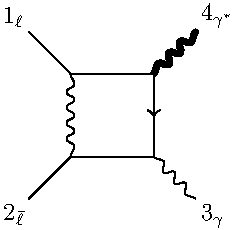
\includegraphics[scale=0.8]{2l2a_1l_a1}
            \caption{$\sal{1}{0}{0}$}
            \label{fig:1Lbox}
        \end{subfigure}
        \begin{subfigure}[c]{0.3\linewidth}
            \centering
            \vspace{4ex}
            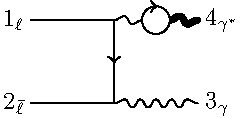
\includegraphics[scale=0.8]{2l2a_1l_a4}
            \vspace{4ex}
            \caption{$\sal{1}{1}{1}$}
            \label{fig:1Lbubble}
        \end{subfigure}
        \\
        \vspace{1em}
        \begin{subfigure}[c]{0.3\linewidth}
            \centering
            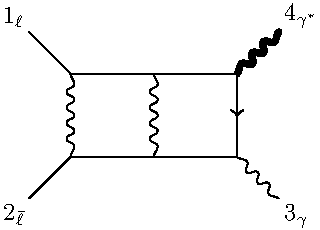
\includegraphics[scale=0.8]{2l2a_2l_a1}
            \caption{$\sal{2}{0}{0}$}
            \label{fig:2Lbox1}
        \end{subfigure}
        \begin{subfigure}[c]{0.3\linewidth}
            \centering
            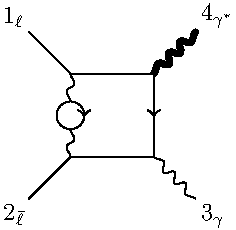
\includegraphics[scale=0.8]{2l2a_2l_a2}
            \caption{$\sal{2}{1}{0}$}
            \label{fig:2Lboxbubble1}
        \end{subfigure}
        \begin{subfigure}[c]{0.3\linewidth}
            \centering
            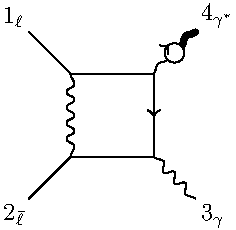
\includegraphics[scale=0.8]{2l2a_2l_a4}
            \caption{$\sal{2}{1}{1}$}
            \label{fig:2Lboxbubble2}
        \end{subfigure}
        \\
        \vspace{1em}
        \begin{subfigure}[c]{0.3\linewidth}
            \centering
            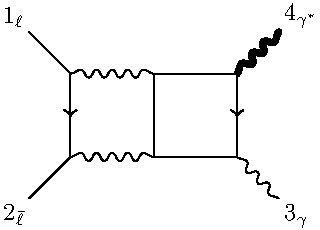
\includegraphics[scale=0.8]{2l2a_2l_a3}
            \caption{$\sal{2}{1}{2}$}
            \label{fig:2Lbox2}
        \end{subfigure}
        \begin{subfigure}[c]{0.3\linewidth}
            \centering
            \vspace{4ex}
            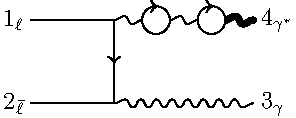
\includegraphics[scale=0.8]{2l2a_2l_a5}
            \vspace{4ex}
            \caption{$\sal{2}{2}{1}$}
        \end{subfigure}
        \caption{
            Representative Feynman diagrams for the subamplitudes defined in \cref{eqQED:nldecomp}.
            The off-shell external leg is indicated by a bold line.
        }
        \label{fig:repr-diagrams}
    \end{center}
\end{figure}

We decompose the loop-level helicity amplitudes $\al{L}$ into gauge-invariant
subamplitudes $\sal{L}{i}{j}$, where the subscript $i$ counts the number of
closed massless fermion loops and $j$ the number of external photons attached
to closed fermion loops. The non-zero contributions are:
\begin{subequations}
    \label{eqQED:nldecomp}
    \begin{align}
        \al{1} &= \sal{1}{0}{0} + \nl \, \sal{1}{1}{1} \,, \\*
        \al{2} &= \sal{2}{0}{0}
        + \nl \left( \sal{2}{1}{0} + \sal{2}{1}{1} + \sal{2}{1}{2} \right)
        + \nl^2 \sal{2}{2}{1} \,,
    \end{align}
\end{subequations}
where $\nl$ denotes the number of charged lepton flavours running in the loops.
Representative Feynman diagrams contributing to these subamplitudes are illustrated in \cref{fig:repr-diagrams}.
Amplitudes with a closed fermion loop attached to an odd number of photons vanish by Furry's theorem.

We decompose the amplitude and subamplitude currents as:
\begin{align}
    \label{eqQED:offshellproj}
    \al{L} = \sum_{k=1}^4 a_{k}^{(L)} \, q_k^\mu \,, \qquad \qquad \sal{L}{i}{j} = \sum_{k=1}^4 a_{i,j;k}^{(L)} \, q_k^\mu \,,
\end{align}
using the following basis written with the spinor-helicity formalism:
\begin{align}
    \label{eqQED:proj-basis}
    q_k^\mu &= p_k^\mu \quad\forall \, k=1,2,3 \,, &
    q_4^\mu &= \frac{\langle 2|p_3p_1\sigma^\mu|2 ] - \langle 1|p_3p_2\sigma^\mu|1 ]}{2 s_{12}} \,.
\end{align}
%Readers not familiar with the spinor-helicity formalism may like to consult one of the many good reviews on the subject~\cite{Mangano:1990by, Dixon:1996wi, Badger:2023eqz}.
Note that $q_4$ is orthogonal to the momenta $p_i$ by construction; one can in fact show that $q_4^\mu\propto \varepsilon^{\mu\nu\rho\sigma}{q_1}_\nu{q_2}_\rho{q_3}_\sigma$. 
The subamplitude coefficients $a_{i,j;k}^{(L)}$ can be related to the amplitude ones $a_{k}^{(L)}$ through \cref{eqQED:nldecomp}.

The scattering amplitudes $\mathcal{M}^{(L)}$ for fully on-shell processes (for instance, for $0 \to e^-e^+ \gamma \mu^-\mu^+$) are obtained by contracting the amplitude currents $\al{L}$ (for $0 \to e^-e^+ \gamma \gamma^*$) with a suitable decay current $\mathcal{V}_\mu$ (in this example, $\gamma^*\to\mu^-\mu^+$) as:
\begin{align}
    \label{eqQED:on-shell-amps}
    \mathcal{M}^{(L)} &\coloneqq \mathcal{A}^{(L)} \cdot\mathcal{V}  = \sum_{k=1}^4 a_k^{(L)} \, \left( q_k\cdot\mathcal{V} \right) \,.
\end{align}
In this manner, the on-shell amplitudes $\mathcal{M}^{(L)}$ are given by the scalar product between the vector of coefficients $(a_1^{(L)}, \ldots, a_4^{(L)})$, and that of decay-vector contractions ${(q_1\cdot\mathcal{V}, \ldots, q_4\cdot\mathcal{V} )}$.
The coefficients $a^{(L)}_k$ depend on the helicities of the three on-shell particles in \cref{eqQED:scatter}, while the decay vector $\mathcal{V}_{\mu}$ depends on the helicities of the particles the off-shell photon decays to. The helicity-summed interference between the $L_1$-loop and the $L_2$-loop matrix elements is then given by:
\begin{align} \label{eqQED:squared_M}
    \mathcal{M}^{(L_1,L_2)} &= \frac{1}{4} \sum_{\vec{h}} {\mathcal{M}^{(L_1)}_{\vec{h}}}^* \mathcal{M}^{(L_2)}_{\vec{h}} \,,
\end{align}
where the subscripts $\vec{h}$ indicates the helicities of all on-shell particles --- that is, including the decay products of the off-shell photon --- and the overall constant factor averages over the helicities of the incoming particles.

The output of the computation described in \cref{secQED:calc} is the set of four projections $\mathcal{A}^{(L)}_{i,j} \cdot q_k$ for each helicity configuration listed in \cref{eqQED:helconfs}.
From these, we determine the subamplitude coefficients $a_{i,j;k}^{(L)}$ by inverting \cref{eqQED:offshellproj} as:
\begin{align}
    \label{eqQED:ampcoeffinv}
    a_{i,j ; k}^{(L)} &= \sum_{m=1}^4 \left(\mathrm{G}^{-1}\right)_{km} \left(\mathcal{A}^{(L)}_{i,j} \cdot q_m\right) \,,
\end{align}
where $\mathrm{G}$ is the Gram matrix of the vectors $q_i$, that is, the matrix of entries $\mathrm{G}_{ij} \coloneqq q_i \cdot q_j$ for $i,j=1,\ldots,4$.
At loop level, we write the subamplitude coefficients as:
\begin{align}
    \label{eqQED:ampprojcoeffs}
    a_{i,j;k}^{(L)} &= \sum_{w=-2L}^{4-2L} \sum_r\,c_{r,w}\,\text{mon}_r(F)\,\eps^w ,
\end{align}
where $\text{mon}_r(F)$ are monomials of special functions $F$ (see \cref{secQED:spec-fns}), and the coefficients $c_{r,w}$ are rational functions of the kinematics. 
We drop the dependence on $i$, $j$, $k$, and $L$ on the right-hand side of \cref{eqQED:ampprojcoeffs} for compactness. 
We truncate the Laurent expansion around $\eps=0$ to the orders required for computing NNLO predictions.
We express the coefficients $c_{r,w}$ as $\mathbb{Q}$-linear combinations of a smaller set of linearly-independent coefficients (see \cref{secQED:calc}).
The analytic expressions of the latter are given explicitly in terms of MTs.
We simplify these expressions through a multivariate partial fraction decomposition using \texttt{MultivariateApart}~\cite{Heller:2021qkz}, and by collecting the common factors.

In the ancillary files~\cite{zenodo}, the directory \texttt{amplitudes/} contains \texttt{Mathematica} files describing the bare helicity subamplitude currents $\sal{L}{i}{j}$ by their coefficients $a_{i,j;k}^{(L)}$ in the form of \cref{eqQED:ampprojcoeffs}.
The \texttt{Mathematica} script \texttt{current.m} is a reference implementation of the numerical evaluation of the bare amplitude coefficients $a_k^{(L)}$ in \cref{eqQED:ampprojcoeffs}, including summation of subamplitudes in \cref{eqQED:nldecomp}, treatment of dependent helicities, and renormalisation scale restoration in \cref{eqQED:scale-restoration}.
The \texttt{Mathematica} script \texttt{evaluation.wl} demonstrates the construction of the five-particle on-shell amplitudes in \cref{eqQED:on-shell-amps} for the process $0\to e^- e^+ \gamma \mu^- \mu^+$, and their helicity-summation to obtain the squared matrix elements in \cref{eqQED:squared_M}.
The results of the script are checked against a reference point included in \texttt{reference\_point.json}.

\smallskip

We perform the following checks of our amplitudes:
\begin{description}
    \item[Ward identity]
        We verify the gauge invariance of the subamplitudes $\sal{L}{i}{j}$ by checking that they vanish on replacing the on-shell photon's polarisation vector with its momentum.

    \item[One-loop crosscheck]
        We successfully crosscheck our one-loop $\nl=0$ helicity-summed matrix element contracted with the decay $\gamma^*\to\mu^-\mu^+$ against the QED NLO electron-line corrections for $e\mu\to e\mu\gamma$ obtained with \texttt{McMule}~\cite{Banerjee:2020rww,ulrich_yannick_2022_6046769}.

    \item[Finite remainder]
      We verify that the $\eps$-poles of the bare amplitudes have the structure predicted by UV renormalisation and IR factorisation~\cite{Catani:1998bh,Gardi:2009qi,Gardi:2009zv,Becher:2009cu,Becher:2009qa}. We then subtract the expected poles and define finite remainders at one and two loops as:
        \begin{subequations}
            \label{eqQED:finite-remainders}
            \begin{align}
                {\mathcal{F}^{(1)}}^\mu &= \left[ \al{1} - \frac{3}{2}\frac{\beta_0}{\eps} \al{0} \right] - Z^{(1)} \al{0} \,,\\
                {\mathcal{F}^{(2)}}^\mu &= \left[ \al{2} - \frac{5}{2}\frac{\beta_0}{\eps} \al{1} - \left(-\frac{15}{8}\frac{\beta_0^2}{\eps^2}+\frac{3}{4}\frac{\beta_1}{\eps}\right) \al{0} \right] - Z^{(2)} \al{0} - Z^{(1)} {\mathcal{F}^{(1)}}^\mu \,,
            \end{align}
        \end{subequations}
        where the square brackets separate renormalisation of UV poles from subtraction of IR poles. The derivation of these formulae follows the procedure outlined in Appendix~\ref{app:QEDpolestructure}. The coefficients $Z^{(L)}$ are given in Appendix~\ref{app:renormconstants}.
\end{description}

\section{Setup of the calculation}
\label{secQED:calc}

In this section, we outline the workflow we used to calculate our amplitudes. For much more detail, we refer the reader to Section~\ref{sec:tools}. Firstly, we generate all Feynman diagrams contributing to \cref{eqQED:scatter} using \texttt{QGRAF}~\cite{Nogueira:1991ex}. Each diagram is then replaced with the corresponding Feynman rules for vertices, propagators, and external states, leading to a collection of $D$-dimensional Feynman integrals. Next, we filter the integrals according to \cref{eqQED:loopdecomp,eqQED:nldecomp} using a collection of \texttt{Mathematica} and \texttt{FORM} scripts~\cite{Kuipers:2012rf,
Ruijl:2017dtg}. Within each subamplitude $\sal{L}{i}{j}$, we then collect the integrals according to their topology, by which we mean a unique set of denominators. 
%For example, the diagrams in \cref{fig:2Lboxbubble1,fig:2Lboxbubble2} belong to different topologies, but those in \cref{fig:2Lbox1,fig:2Lbox2} belong to the same topology (under the assumption of massless lepton propagators). 
At this point, the subamplitudes are sums of Feynman integrals over distinct integral topologies, with the numerators given by linear combinations of monomials that depend on the loop as well as the external momenta. To work with the projected helicity subamplitudes $\am^{(L)}_{i,j}\cdot q_k$, we specify the polarisations of external particles according to \cref{eqQED:helconfs}, as well as the projector $q_k^\mu$ of the off-shell photon from \cref{eqQED:proj-basis}. It is natural to express helicity-dependent objects using the spinor-helicity formalism. Then, the monomials of loop momenta contain the following scalar products and spinor strings:
\begin{equation} \label{eqQED:loopmomobjects}
	\left\{ k_i \cdot k_j, \,
    k_i \cdot p_j ,\,
    \braket{ij},\,
    \braketsq{ij},\,
    \langle i |k_i |j],\,
    \langle i |p_4 |j],\,
    \bra{i}k_i p_4\ket{j},\,
    [i| k_i p_4 |j] \right\} \,.
\end{equation}
Their coefficients, on the other hand, are composed of the same type of
objects, but do not contain any dependence on loop momenta $k_i$.  Similarly to our previous work, we express these coefficients using the rational parametrisation in terms of MTs. The single-off-shell four-particle phase space $p$ is obtained from a massless five-particle parametrisation $q$ (defined in Appendix A of~\incite{Badger:2021imn} with $\{x_2\leftrightarrow x_4,x_3\leftrightarrow x_5\}$) under:
\begin{align}
    p_i &= q_i \qquad \forall i=1,2,3, & p_4=q_4+q_5 \, .
\end{align}
The MTs $x_i$ are then related to the scalar invariants $\vec{s}$ through:
\begin{align} \label{eqQED:mtvs}
    s_{12} &= x_1 \,, &
    s_{23} &= x_1 x_2 \,, &
    s_4 &= x_1 x_3 \,.
\end{align}
The phase information for the helicity configurations of \cref{eqQED:helconfs} is restored using the following phase factors: 
\begin{align}
  \Phi(-++) &= \frac{\langle 1 2 \rangle}{\langle 2 3 \rangle^2} \,,&
  \Phi(-+-) &= \frac{[ 1 2 ]}{[ 1 3 ]^2} \,,
\end{align}
which in our momentum twistor parameterisation are given by:
\begin{align}
  \Phi(-++) &= x_1^2 \,,&
  \Phi(-+-) &= - \frac{1}{x_1 (1 + x_2 - x_3)^2}   \,.
\end{align}
We refer to Appendix~C of \incite{Badger:2023mgf} for a thorough discussion of how to restore the phase information in a momentum twistor parameterisation.
  
%The goal of this approach is to sidestep the algebraic complexity which typically plagues the intermediate stages of symbolic computations by evaluating numerically all rational coefficients. Using integers modulo some large prime number ---~which constitute a finite field~--- for the numerical evaluation allows us to avoid the loss of accuracy inherent to floating-point numbers, as well as the expensive arbitrary-precision arithmetic required by rational numbers.  Manipulations needed to further process the rational coefficients are a completely separate problem from the calculation of the integrals or special functions that these coefficients multiply. In fact, they can be implemented as a series of rational transformations over finite fields. We stress that this is the methodology we follow at each step of the computation described below. In particular, we use the package \texttt{FiniteFlow}~\cite{Peraro:2019svx}, which is conveniently interfaced to \texttt{Mathematica}. The analytic form of the coefficients is not known at any intermediate step. It is reconstructed from the finite-field samples only at the very end of the workflow.

\begin{figure}
    \begin{center}
        \begin{subfigure}[c]{\linewidth}
            \centering
            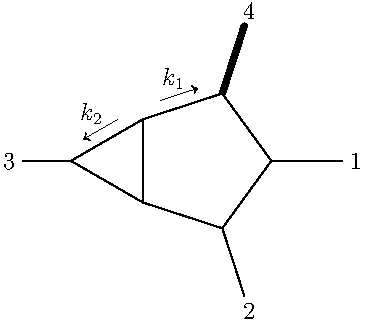
\includegraphics[scale=0.8]{pentatriangle_m1}
            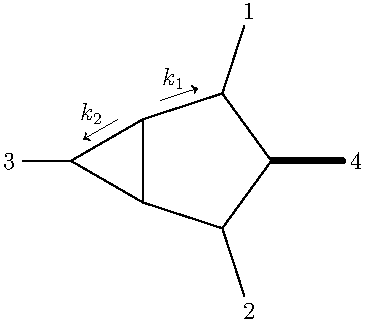
\includegraphics[scale=0.8]{pentatriangle_m2}
            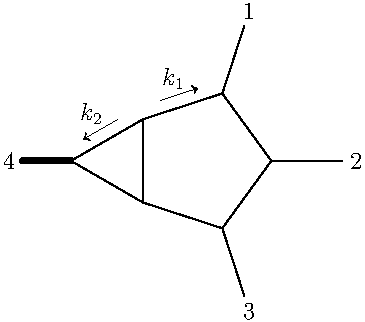
\includegraphics[scale=0.8]{pentatriangle_m4}
            \caption{Penta-triangles}
            \label{fig:pentatriangle}
        \end{subfigure}
        \\
        \vspace{1em}
        \begin{subfigure}[c]{0.3\linewidth}
            \centering
            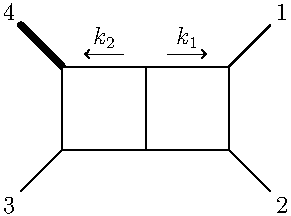
\includegraphics[scale=0.8]{doublebox_m4}
            \caption{Double-box}
            \label{fig:double-box}
        \end{subfigure}
        \begin{subfigure}[c]{0.6\linewidth}
            \centering
            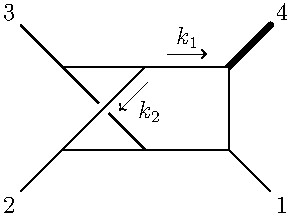
\includegraphics[scale=0.8]{crosseddoublebox_m1}
            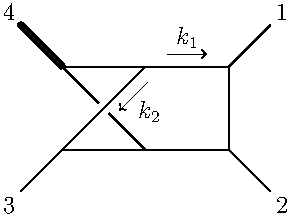
\includegraphics[scale=0.8]{crosseddoublebox_m4}
            \caption{Crossed double-boxes}
            \label{fig:crosseddouble-box}
        \end{subfigure}
    \end{center}
    \caption{ 
        The two-loop amplitudes include six ordered integral families: three penta-triangles, a double-box, and two crossed double-boxes.
        All are planar except for the crossed double-boxes.
        The off-shell external leg is indicated by a bold line.
        External legs have outgoing momenta.
    }
    \label{fig:int-fams}
\end{figure}
This marks the start of our finite-field sampling
procedure~\cite{Peraro:2016wsq}. 
%Firstly, we note that not all integral topologies are independent: some of them can be written as subtopologies of others. 
Firstly, we define the set of maximal topologies, i.e.~topologies with the maximum number of propagators allowed for $L$-loop, $n$-particle diagrams. In Fig.~\ref{fig:int-fams}, we present the maximal topologies for the process under consideration in an arbitrary ordering of the external momenta (we give their explicit definitions in \cref{app:int_def}). Several orderings of the external momenta are relevant for the amplitudes, and we treat them as distinct families. Next, we map all topologies present so far onto one of these maximal topologies. The loop momenta dependent objects of \cref{eqQED:loopmomobjects} are then expressed through the nine inverse propagators and ISPs associated with the chosen maximal topology. In this way, each subamplitude is now a sum of integrals compatible with IBP reduction~\cite{Tkachov:1981wb,Chetyrkin:1981qh}, while their coefficients depend purely on external kinematics. We generate the required IBP relations using \texttt{LiteRed}~\cite{Lee:2012cn}. The resulting IBP system is then solved using the Laporta algorithm~\cite{Laporta:2001dd} with \texttt{FiniteFlow}'s linear solver to yield the reduction of all the integrals present within our maximal topologies onto a much smaller subset of MIs. We choose the MIs such that they satisfy DEs in canonical form~\cite{Henn:2013pwa} (see \cref{secQED:basis_construction}). 

In many amplitude applications, multiple permutations of the ordered topologies (such as the ones in Fig.~\ref{fig:int-fams}) can appear. In this case, it might be beneficial to use an optimised strategy for the IBP reduction which performs the reduction in the ordered families only and then permutes the solutions onto the desired `unordered' families. This permutation can be implemented numerically within finite fields, thus avoiding the need to work with large analytic IBP solutions. Overall, this approach allow us to reduce the time and memory consumption required for the IBP reduction stage, which often proves to be the bottleneck of the whole computation. We describe this strategy in detail in Appendix~\ref{app:altIBPs}.

After the IBP reduction, each projected helicity subamplitude $\am^{(L)}_{i,j}\cdot q_k$
is written as a linear combination of MIs multiplied by rational
coefficients of $\eps$ and the kinematic variables. We now write the MIs
in terms of a basis of special functions up to the required order in $\eps$
(see \cref{secQED:spec-fns}). Finally, we Laurent expand the amplitude around
$\eps=0$, the deepest pole being $1/\eps^{2 L}$ at $L$ loops. The only step
left is to reconstruct the rational coefficients of the special-function
monomials from their samples over finite fields. To simplify this task, we employ chosen strategies already described in Section~\ref{Hbbsec:reduction}.
%In general, this might be a daunting challenge and its complexity stems from two separate factors. The workflow described so far is a series of rational operations chained together within a so-called dataflow graph~\cite{Peraro:2019svx}. As such, we essentially have a black-box algorithm which takes numerical values of the kinematic variables as input, and returns the corresponding numerical values of the rational coefficients of the special-function monomials. The first factor is that several sample points are necessary to infer the analytic expression of these coefficients from their values in the finite fields. The required number is correlated with the polynomial degrees of the rational functions viewed as ratios of polynomials: the higher the degree, the more sample points are required. The second factor affecting the reconstruction complexity is the time it takes to obtain the values of the coefficients at each sample point. The more complicated the dataflow graph is, i.e.~the more operations are chained together and the more difficult each operation is, the longer it will take to run the black-box algorithm. The most expensive operation in this regard is the evaluation of the solution to the IBP system.  The total reconstruction
%time can thus be estimated as:
%\begin{equation} \label{eqQED:rectimeschematic}
%	\text{reconstruction time} \approx (\text{number of sample points}) \times %(\text{evaluation time per point})\,.
%\end{equation}
%We emphasise that the sample evaluations can be run in parallel. For a detailed discussion of various strategies to improve the reconstruction time, see section~4 of \incite{Badger:2021imn} and section~3.5 of \incite{Badger:2022ncb}. Here, we give a brief overview of the tools that proved sufficient for this work.
Specifically, we look for $\mathbb{Q}$-linear relations among the rational
coefficients of each helicity subamplitude, which allows us to select those coefficients for reconstruction which have the lowest degrees. Then, we employ the technique of matching the denominators of the rational coefficients against an ansatz. Here, we use the following factors:
\begin{equation}
	\left\{\braket{ij} , \, \braketsq{ij} , \, \bra{i}p_4|j] , \, s_{ij} - s_{k4} , \, s_{i4} - s_4 , \, s_4 \right\} \,,
\end{equation}
for all $i, j, k = 1, 2, 3$ such that $i\neq j \neq k$. This list includes denominator factors of the DEs satisfied by the MIs (listed by \cref{eqQED:alphabet}), 
as well as spinor structures aimed at capturing the phase information of helicity amplitudes.
%We then determine the exponents of the ans\"atze by comparing them to the coefficients reconstructed on a univariate slice of the kinematic variables~\cite{Abreu:2019odu}, which are very cheap to obtain. We find that with this ansatz it is possible to determine all denominator factors ---~which indeed are linked to the singularity structure of the amplitude~--- and sometimes also some numerator factors. As a result, the undetermined functions yet to be reconstructed are of lower degree and require fewer sample points. 
We reconstruct the analytic form of the remaining rational functions using \texttt{FiniteFlow}'s built-in multivariate functional reconstruction algorithm.

Finally, we note that, for more computationally demanding processes, further simplification strategies can be used. We refer the reader to Section~\ref{wyjsec:Simplification} and \incites{Badger:2021imn, Badger:2021ega, Badger:2022ncb, DeLaurentis:2022otd, Badger:2023mgf, Abreu:2023bdp, Liu:2023cgs}.

\section{Computation of the \aclp{MI}}
\label{secQED:spec-fns}

The MIs for the relevant integral families were computed analytically in \incites{gehrmann:2000zt,gehrmann:2001ck,Gehrmann:2023etk} (see also~\incite{Gehrmann:2002zr} for a thorough discussion of the analytic continuation).
We revisit this computation to obtain expressions for the MIs which are better suited for the amplitude-computation workflow discussed in \cref{secQED:calc}. To this end, we compute the MIs for \emph{all permutations} of the external legs in terms of a \emph{basis} of special functions, following the approach of \incites{Gehrmann:2018yef,Chicherin:2020oor,Badger:2021nhg,Chicherin:2021dyp,Abreu:2023rco}. In other words, we express all the Feynman integrals contributing to the amplitudes in terms of a set of special functions which are algebraically independent. Having such a unified and unique representation for all permutations of the integral families allows for simplifications and cancellations among different permutations of the Feynman integrals. This leads to a simpler expression of the amplitudes and to a more efficient functional reconstruction in the finite-field setup presented in \cref{secQED:calc}. We emphasise that our results cover all MIs required for computing \emph{any} two-loop four-particle amplitude with a single external off-shell leg, and not just the ones required for the amplitudes presented in this work.

We discuss the construction of the basis in \cref{secQED:basis_construction}, and how we express it in terms of GPLs in \cref{secQED:basis_MPLs}. 
Finally, we give some details about the numerical evaluation and the checks we performed in \cref{secQED:performance}.


\subsection{Construction of the special function basis}
\label{secQED:basis_construction}

We follow the strategy presented in \incite{Abreu:2023rco}. The starting point are the DEs satisfied by the MIs for each family~\cite{Barucchi:1973zm, KOTIKOV1991158, KOTIKOV1991123, Gehrmann:1999as, Bern:1993kr}. Let $T$ label an integral family, e.g.\ the double-box in \cref{fig:double-box} for an arbitrary permutation of the external massless momenta. We choose a basis of \emph{pure} master integrals $\vv{\text{MI}}_T$, that is, a basis which satisfies DEs in the canonical form~\cite{Henn:2013pwa}:
\begin{align}
\label{eqQED:canonicalDEs}
\dd \vv{\text{MI}}_T(\vec{s}; \eps) = \eps \, \left( \sum_{i=1}^{7} A^{(T)}_i \, \dd \log w_i(\vec{s}) \right) \cdot \vv{\text{MI}}_T(\vec{s}; \eps) \,.
\end{align}
Here, $\dd$ is the total differential, $\dd f \coloneqq \dd s_{12} \, \partial_{s_{12}} f + \dd s_{23} \, \partial_{s_{23}} f +  \dd s_{4} \, \partial_{s_{4}} f $, $A^{(T)}_i$ are constant $\left(|\text{MI}_T| \times |\text{MI}_T|\right)$ matrices, with $|\text{MI}_T|$ the number of MIs of the family $T$, and: 
\begin{align}
\label{eqQED:alphabet}
\begin{alignedat}{4}
& w_1 = s_{12} \,, 
&& w_2 = s_{23} \,, 
&& w_3 = s_{12} + s_{23} \,, \qquad
&& w_4 = s_{12} - s_4 \,,  \\
& w_5 = s_{23} - s_4 \,, \qquad
&& w_6 = s_{12} + s_{23} - s_4 \,, \qquad
&& w_7 = s_4 \, &&
\end{alignedat}
\end{align}
are the `letters'. We find such canonical bases by a mixture of methods: the package \texttt{DlogBasis}~\cite{Henn:2020lye}, the analysis of results in the literature for related integral families (massless two-loop five-point planar integrals~\cite{Gehrmann:2015bfy} and two-loop four-point integrals with two massive external legs~\cite{Henn:2014lfa,Caola:2014lpa}), and a set of heuristic rules (see e.g.\ \incite{Dlapa:2022nct}).
We normalise the MIs such that their expansion around $\eps=0$ starts from order $\eps^0$:
\begin{align}
\vv{\text{MI}}_T(\vec{s} ; \eps) = \sum_{k \ge 0} \eps^k \, \vv{\text{MI}}_T^{(k)}(\vec{s}) \,.
\end{align}
For the purpose of computing two-loop scattering amplitudes up to their finite part (i.e., up to order $\eps^0$), it suffices to restrict our attention to $k \le 4$.
Since the MIs satisfy canonical DEs, Eq.~\ref{eqQED:canonicalDEs}, the $\eps$-order of the MI coefficients $\vv{\text{MI}}_T^{(k)}(\vec{s})$ equals their transcendental weight~\cite{Henn:2013pwa}.
We compute the derivatives of the MIs using \texttt{FiniteFlow}~\cite{Peraro:2019svx} and \texttt{LiteRed}~\cite{Lee:2012cn}.
We do so only for the integral families with the ordering of the external momenta shown in \cref{fig:int-fams}, and obtain those for all other orderings of the external massless legs by permutation. 
We provide the definition of the pure MIs and the corresponding DEs for all one- and two-loop four-point one-mass families in \cref{fig:int-fams} in the folder \texttt{pure\_mi\_bases/} of our ancillary files~\cite{zenodo}. 

In order to solve the DEs in Eq.~\ref{eqQED:canonicalDEs} we need boundary values, i.e., values of all MIs up to order $\eps^4$ at a phase-space point. 
Due to the simplicity ---~by today's standards~--- of the integrals under consideration, an arbitrary (non-singular) phase-space point would do. 
Nonetheless, we make a more refined choice following some of the criteria of \incites{Chicherin:2020oor,Chicherin:2021dyp}.
We choose the following point in the $s_{12}$ channel (see \cref{app:an_cont}),
\begin{align} \label{eqQED:s0}
\vec{s}_0 = \left( 2, \, -\frac{1}{2}, \, 1 \right) \,,
\end{align}
motivated by two principles: that it is symmetric under the permutations which preserve the $s_{12}$ channel (i.e., swapping $p_1 \leftrightarrow p_2$), and that it contains few distinct prime factors.
The first condition reduces the number of permuted integral families we need to evaluate in order to obtain the boundary values.
The second condition reduces the number of independent transcendental constants appearing in the boundary values, which simplifies the construction of the basis of special functions. 
The order-$\eps^0$ boundary values $\vv{\text{MI}}_T^{(0)}$ are rational constants. We obtain them up to their overall normalisation by solving the `first-entry conditions'~\cite{Gaiotto:2011dt}, i.e., by requiring the absence of unphysical branch cuts in the solutions. We fix the overall normalisation and the higher-order boundary values $\vv{\text{MI}}_T^{(k)}(\vec{s}_0)$ (for $1\le k\le 4$) by evaluating all MIs with \texttt{AMFlow}~\cite{Liu:2022chg} (interfaced to 
\texttt{FiniteFlow}~\cite{Peraro:2019svx} and \texttt{LiteRed}~\cite{Lee:2012cn}) at $\vec{s}_0$ with at least $60$-digit precision.
We anticipate from \cref{secQED:basis_MPLs} that, although we use floating-point boundary values, our results in terms of GPLs are fully~analytic. 

The canonical DEs in Eq.~\ref{eqQED:canonicalDEs} and the boundary values for all integral families are the input for the algorithm of \incite{Abreu:2023rco} for constructing a basis of special functions. We refer to the original work for a thorough discussion. 
Out of all MI coefficients up to transcendental weight $4$, the algorithm selects a subset, denoted $F \coloneqq \{F^{(k)}_i(\vec{s})\}$, which satisfy two constraints. 
First, they are \emph{algebraically independent}, that is, there are no polynomial functional relations among them. Second, the MI coefficients of all families (including all permutations of the external massless legs) up to transcendental weight $4$ are expressed as polynomials in the $\{F^{(k)}_i(\vec{s})\}$ and the zeta values $\zeta_2 = \pi^2/6$ and $\zeta_3$. For example, an arbitrary weight-$2$ MI coefficient $\text{MI}^{(2)}(\vec{s})$ has the general form
\begin{align}
\text{MI}^{(2)}(\vec{s}) = \sum_{i=1}^{4} c_i \, F_i^{(2)}(\vec{s}) + \sum_{i \le j =1}^{3} d_{ij} \, F_i^{(1)}(\vec{s}) \,  F_j^{(1)}(\vec{s}) + e \, \zeta_2 \,,
\end{align}
with $c_i, d_{ij}, e \in \mathbb{Q}$. This special subset of MI coefficients, $\{F^{(k)}_i(\vec{s})\}$, constitutes our special function basis. 
We give the number of functions in the basis in \cref{tab:func_basis}. Note that there is freedom in the choice of which MI coefficients make up the basis. We make use of this freedom to choose as many basis-elements as possible from the one-loop family, then complement them with coefficients from the planar two-loop families, and finally complete them with coefficients from the non-planar two-loop families. In this way no two-loop MI coefficients appear in the one-loop amplitudes, and no non-planar two-loop MI coefficients appear in those amplitudes where only planar diagrams contribute (as is often the case in the leading colour approximation of QCD).

\begin{table}
    \centering
    \begin{tabular}{cc}
        \hline
        Weight & Number of basis functions \\
        \hline
        $1$ & 4 \\
        $2$ & 3 \\
        $3$ & 20 \\
        $4$ & 67 \\
        \hline
    \end{tabular}
    \caption{Number of functions $\{F^{(k)}_i\}$ in the basis weight by weight.}
    \label{tab:func_basis}
\end{table}

The folder \texttt{mi2func/} of our ancillary files~\cite{zenodo} contains the expression of all MI coefficients (for all one- and two-loop integral families in all permutations of the external massless legs) up to weight $4$ in terms of our special function basis. This result enables the efficient amplitude-computation strategy based on finite-field arithmetic discussed in \cref{secQED:calc}.
However, at this stage the basis functions $\{F^{(k)}_i\}$ are expressed in terms of CIIs~\cite{Chen:1977oja} and numerical boundary values $\vv{\text{MI}}^{(k)}(\vec{s}_0)$. This representation is excellent for investigating the analytic properties of Feynman integrals and amplitudes, but it is not readily suitable for an efficient numerical evaluation.
In the next section we discuss how we construct a representation of the function basis in terms of GPLs and zeta values, which is well suited for an efficient and stable numerical evaluation.


\subsection{Expression in terms of GPLs}
\label{secQED:basis_MPLs}

In this section, we construct a representation of our function basis in terms of GPLs (see Section~\ref{sec:DEdlogform} for their definition). %The weight-$n$ GPL of indices $\{a_1,\ldots,a_n\}$ and argument $x$ is defined recursively as
%\begin{align} 
%G(a_1,a_2,\ldots,a_n; x) \coloneqq \int_0^x \frac{\dd t}{t - a_1} \, G(a_2,\ldots,a_n; t) \,, \qquad a_n \neq 0 \,, 
%\end{align}
%for $a_n \neq 0$, starting with $G(;x) = 1$. Trailing zeros, i.e., zeros in the right-most indices, are allowed through the definition
%\begin{align} \label{eqQED:trailingzeros}
%G(\underbrace{0,\ldots,0}_{k}; x) \coloneqq \frac{1}{k!} \log^k(x) \,.
%\end{align}
%We refer to \incite{Vollinga:2004sn} for a thorough discussion.
Since the letters in \cref{eqQED:alphabet} are rational and linear in all variables, we can solve the canonical DEs in \cref{eqQED:canonicalDEs} algorithmically in terms of GPLs. Order by order in $\eps$, the solution is given~by:
\begin{align} \label{eqQED:solution}
\vv{\text{MI}}_T^{(k)}(\vec{s}) = \sum_{i=1}^7 A_i^{(T)} \cdot \int_{\gamma} \dd \log \bigl(w_i(\vec{s}=\gamma) \bigr) \,\vv{\text{MI}}_T^{(k-1)}\bigl(\vec{s}=\gamma\bigr) + \vec{b}^{(k)}_{T} \,,
\end{align}
starting from the constant weight-$0$ boundary values $\vv{\text{MI}}_T^{(0)}$ determined in the previous subsection. Here, $\gamma$ is a path connecting an arbitrary base-point $\vec{s}_{\mathrm{base}}$ to the end-point $\vec{s}$. The weight-$k$ constants $\vec{b}^{(k)}_{T} $ are given by the values of the integrals at the base-point, $ \vec{b}^{(k)}_{T} = \vv{\text{MI}}_T^{(k)}(\vec{s}_{\mathrm{base}})$.
For $\vec{s}_{\mathrm{base}}$ we may use the boundary point $\vec{s}_0$ in \cref{eqQED:s0}, so that the constants $\vec{b}^{(k)}_{T}$ coincide with the boundary values determined numerically in the previous section. We follow a different approach, which allows us to trade all numerical constants in the expressions for zeta values.

We find it convenient to change variables from $(s_{12},s_{23},s_4)$ to $(z_1,z_2,s_4)$, with:
\begin{align}
z_1 = \frac{s_{12}}{s_4} \,, \qquad \qquad z_2 = \frac{s_{23}}{s_4} \,.
\end{align}
This way, there is only one dimensionful variable, $s_4$, the dependence on which is fixed as an overall factor by dimensional analysis.
We then integrate the canonical DEs as in \cref{eqQED:solution} along the following piece-wise path in the $(z_1,z_2,s_4)$ space:
\begin{align} \label{eqQED:path}
(0,0,0) \overset{\gamma_1}{\longrightarrow} (z_1, 0, 0)  \overset{\gamma_2}{\longrightarrow} (z_1, z_2, 0)  \overset{\gamma_3}{\longrightarrow} (z_1, z_2, s_4) \,.
\end{align}
Since the Feynman integrals are divergent at the chosen base-point, the latter is understood in a \emph{regularised} sense (we refer to section~4 of \incite{Abreu:2022mfk} for a thorough discussion).
Choosing $(0,0,0)$ as base-point has the important benefit of removing spurious transcendental numbers that would pollute the solution were we to choose a base-point where the integrals are finite. As we will see below, only zeta values appear.
Roughly speaking, we define regularised, finite values $\vec{b}^{(k)}_{T} \coloneqq \mathrm{Reg} \, \vv{\text{MI}}_T^{(k)}(\vec{s}_{\mathrm{base}})$ by introducing a regulator and formally setting to $0$ the (divergent) logarithms of the regulator.
Since the integrals are finite at a generic end-point $\vec{s}$, the divergences at the base-point must cancel out with divergences arising in the integration. We can thus drop all these divergences. Provided that we do it consistently between the integration and the base-point values $\vec{b}^{(k)}_{T}$, this leads to a finite and unique result. In practice, we fix the finite base-point values $\vec{b}^{(k)}_{T}$ by matching the solution $\vv{\text{MI}}_T^{(k)}(\vec{s})$ evaluated at the boundary point $\vec{s}_0$ against the boundary values discussed in the previous subsection. 

We therefore keep the $\vec{b}^{(k)}_{T}$ as symbols and integrate the canonical DEs as in \cref{eqQED:solution} along the path in \cref{eqQED:path} up to weight $4$. 
We parameterise each piece of the path in \cref{eqQED:path} linearly. For instance, 
$\gamma_2(t) = ( z_1,  t  , 0 )$,
with $t \in [0,z_2]$.
\begin{itemize}
\item The $\gamma_1$ integration leads to GPLs with indices in $\{0,1\}$ and argument~$z_1$.
\item The $\gamma_2$ integration leads to GPLs with indices in $\{0,1, 1-z_1, -z_1\}$ and argument~$z_2$.
\item The $\gamma_3$ integration leads to powers of $\log(-s_4)$, fixed by dimensional analysis.
\end{itemize}
Once we have obtained expressions for all MIs in terms of GPLs and symbolic constants $\vec{b}^{(k)}_T$, we equate them to the numerical boundary values at $\vec{s}_0$, and solve for the $\vec{b}^{(k)}_{T}$. We use \texttt{GiNaC}~\cite{Bauer:2000cp,Vollinga:2004sn} to evaluate the GPLs numerically.
Finally, we use the \texttt{PSLQ} algorithm~\cite{PSLQ} to express the ensuing values of $\vec{b}^{(k)}_{T}$ in terms of $\zeta_2$ and $\zeta_3$. As a result, we obtain a fully analytic representation of all MIs --- and thus of our special function basis $\{F^{(k)}_i\}$ --- in terms of GPLs and zeta values, up to weight $4$.

Contrary to the functions in the basis $\{F^{(k)}_i\}$, the GPLs in their representation satisfy functional relations. We make use of this freedom to optimise our expressions in view of their numerical evaluation by reducing the number of distinct GPLs that need to be evaluated. First, we use the shuffle algebra of GPLs to push all trailing zeros into logarithms through \cref{eq:GPLtologzero}. Next, we employ the scaling relation:
\begin{align}
G(a_1, \ldots, a_n; x) = G\left(\frac{a_1}{x}, \ldots, \frac{a_n}{x}; 1\right) \,,
\end{align}
which holds for $x, a_n \neq 0$. As a result, all GPLs have argument $1$ and indices:
\begin{align} \label{eqQED:indices}
l_0 = 0 \,, \qquad 
l_1 = \frac{s_4}{s_{12}} \,, \qquad 
l_2 = \frac{s_4}{s_{23}} \,, \qquad
l_3 = \frac{s_4-s_{12}}{s_{23}} \,, \qquad
l_4 = - \frac{s_{12}}{s_{23}}\,.
\end{align}
%
Finally, we decompose the GPLs to \emph{Lyndon words}~\cite{Radford1979ANR} using \texttt{PolyLogTools}~\cite{Duhr:2019tlz}; we refer to the latter work for a thorough explanation, and give here only a simple example. 
This procedure requires that we choose a symbolic ordering of the GPL indices. We choose $l_0 \prec l_1 \prec l_2 \prec l_3 \prec l_4$, meaning that $l_1$ is greater than $l_0$, and so on. 
Consider the GPL $G(l_1, l_0; 1)$, whose indices are not sorted according to the ordering above, since $l_1 \succ l_0$. We can use the shuffle algebra of GPLs to rewrite it in terms of GPLs whose indices are sorted according to the chosen ordering:
\begin{align}
G(l_1, l_0; 1) = G(l_0;1) \, G(l_1;1) - G(l_0, l_1; 1) \,.
\end{align}
Doing this consistently throughout all expressions reduces the number of higher-weight GPLs in favour of products of lower-weight ones, which are cheaper to evaluate numerically. To maximise the impact in this sense, we tested all possible orderings of the indices and selected the one --- given above --- which minimises the number of weight-4 GPLs.
The resulting representation of the function basis contains $4$ weight-1, 6 weight-2, 19 weight-3, and 25 weight-4 GPLs, as well as $3$ logarithms: 
\begin{align} \label{eqQED:logs}
\log(s_{12}/s_4) \,, \qquad \quad \log(s_{23}/s_4) \,, \qquad \quad \log(-s_4) \,.
\end{align}
We write the latter in terms of logarithms rather than GPLs as they play an important role in the factorisation of the IR divergences in the scattering amplitudes (see \cref{app:QEDpolestructure} for the IR structure of the amplitudes we compute here). We stress that $\log(-s_4)$ is the only function of a dimensionful argument in our representation of the function basis. 

We provide in the folder \texttt{mi2func/} of our ancillary files~\cite{zenodo} the expression of the basis functions $\{F^{(k)}_i\}$ in terms of GPLs, logarithms, $\zeta_2$ and $\zeta_3$.

\smallskip

It is important to stress that the GPLs are multi-valued functions.
For unit argument, there is a pole on the integration contour whenever one of the indices lies between $0$ and $1$. In this case the contour must be deformed in the complex plane, either above or below the pole, leading to different branches. Our GPLs are thus well-defined only in the 
kinematic region where all GPL indices in \cref{eqQED:indices} are either less than 0 or greater than 1, and $s_4 < 0$ for the argument of all logarithms in \cref{eqQED:logs} to be positive. We discuss how to analytically continue the GPLs and the logarithms in \cref{eqQED:logs} to the kinematic regions of interest in \cref{app:an_cont}.



\subsection{Performance and validation}
\label{secQED:performance}

We validated our results for the MIs of all families by crosschecking them against values obtained with \texttt{AMFlow}~\cite{Liu:2022chg} at several random points in all the physical kinematic regions discussed in \cref{app:an_cont}. Furthermore, we find agreement with the results of~\incite{Gehrmann:2023etk}. We employ \texttt{GiNaC}~\cite{Bauer:2000cp,Vollinga:2004sn} to evaluate the GPLs.

Our results allow for an efficient and stable evaluation of the MIs, and are thus ready for immediate deployment in phenomenology. Indeed, the amplitudes we computed in this work have already been implemented in \texttt{McMule}~\cite{Banerjee:2020rww,ulrich_yannick_2022_6046769} to provide the \acl{RVV} electron-line corrections  $e \mu \to e \mu$ scattering. The evaluation is efficient, running at $\approx 130$ events per second in the bulk of the phase space~\cite{ulrich-radcor} using \texttt{handyG}~\cite{Naterop:2019xaf} for the evaluation of the GPLs.

\end{document}